\documentclass[a4paper,12pt]{article} % тип документа

%  Русский язык
\usepackage{mathtext}               % русский язык в формулах
\usepackage[T2A]{fontenc}			% кодировка
\usepackage[utf8]{inputenc}			% кодировка исходного текста
\usepackage[english,russian]{babel}	% локализация и переносы

\usepackage{graphicx}               % импорт изображений
\usepackage{wrapfig}                % обтекаемые изображения
\graphicspath{{pictures/}}          % обращение к подкаталогу с изображениями
\usepackage{amsfonts}               % буквы с двойными штрихами
\usepackage{indentfirst}            % indent first
\usepackage{amsmath}                % можно выводить фигурные скобочки -- делать системы уравнений
\usepackage[table,xcdraw]{xcolor}   % таблицы
\usepackage{amsmath,amsfonts,amssymb,amsthm,mathtools} % Математика
\usepackage{wasysym}                % ???
\usepackage{upgreek}                % ???  

\usepackage{gensymb} % degree symbol
\usepackage{mathrsfs}

\usepackage{tikz}
\usetikzlibrary{graphs,graphs.standard}

\usepackage{cancel} % перечеркивания

%% Интервалы
\linespread{1}
\usepackage{multirow}

%% Перенос знаков в формулах (по Львовскому)
\newcommand*{\hm}[1]{#1\nobreak\discretionary{}
	{\hbox{$\mathsurround=0pt #1$}}{}}

%% Русские списки
\usepackage{enumitem}
\makeatletter
\AddEnumerateCounter{\asbuk}{\russian@alph}
\makeatother

% Дополнительная работа с математикой
\usepackage{amsmath,amsfonts,amssymb,amsthm,mathtools} % AMS
\usepackage{icomma} % "Умная" запятая: $0,2$ --- число, $0, 2$ --- перечисление

\usepackage{dsfont}
\usepackage{cancel} % перечеркивания

%%% Свои команды
\DeclareMathOperator{\sgn}{\mathop{sgn}}

%%% Программирование
\usepackage{etoolbox} % логические операторы

\usepackage{marvosym}
\usepackage{wasysym}

%%% Страница
\usepackage{extsizes} % Возможность сделать 14-й шрифт
\usepackage{geometry} % Простой способ задавать поля
	\geometry{top=20mm}
	\geometry{bottom=20mm}
	\geometry{left=20mm}
	\geometry{right=20mm}
	
\usepackage{mathrsfs}

\newcommand{\eqdef}{\stackrel{\mathrm{def}}{=}}
\newcommand{\ryad}{\sum\limits^{\infty}_{k = 0}}

\newcommand{\R}{\mathbb{R}}
\newcommand{\N}{\mathbb{N}}
\newcommand{\series}{\sum\limits_{k=1}^{\infty}}
\newcommand{\useries}{\sum\limits_{k=1}^{\infty} u_k}
\newcommand{\useriesl}{\sum\limits_{k=1}^{\infty} u_k < \infty}
\newcommand{\useriese}{\sum\limits_{k=1}^{\infty} u_k = \infty}
\newcommand{\auseries}{\sum\limits_{k=1}^{\infty} |u_k|}
\newcommand{\auseriesl}{\sum\limits_{k=1}^{\infty} |u_k| < \infty}
\newcommand{\auseriese}{\sum\limits_{k=1}^{\infty} |u_k| = \infty}
\newcommand{\sn}{\sum\limits_{k=1}^{n} u_k}

\renewcommand {\ge}{\geqslant}
\renewcommand {\le}{\leqslant}
\renewcommand {\geq}{\geqslant}
\renewcommand {\leq}{\leqslant}
\renewcommand {\epsilon}{\varepsilon}

\usepackage{titlesec}
\titlelabel{\thetitle.\quad}
%%% Для точек после названий секций

\usepackage{hyperref}
%%% Настройка ссылок
\hypersetup
{
	colorlinks = true,
	linkcolor  = black,
	filecolor  = magenta,
	urlcolor   = blue
}
%%% Конец настройки ссылок


\begin{document}

%=======================================================================================

\begin{titlepage}
\begin{center}
\
\vfill

{\LARGE \textsc{\textbf{Парашютист без парашюта: \\неодим, воздух и... медные трубы.\\}}}

\vspace{2em}

Гончаренко Валентина, 2 курс ФРКТ, группа Б01-009

\vfill

Декабрь 2021
\end{center}
\end{titlepage}

%=======================================================================================

\newpage
\tableofcontents{} %содержание
\newpage

%1
%=======================================================================================

\section{Введение}

Многие люди мечтают попробовать прыжок с парашютом: свобода, адреналин, вид на пейзаж с высоты птичьего полёта и плавное приземление. Развлечение, однако, весьма опасное -- всегда есть риск, что что-то пойдет не по плану. А вот для неодима этот план работает в ста процентах случаев <<прыжков>> -- магнит в окружении проводника безошибочно раскрывает невидимый парашют -- все по канонам Максвелла, Фарадея и Фуко.

В данной работе исследуется явление возникновения вихревых токов в медных трубах при прохождении сквозь них неодимового магнита. Визуально эффект проявляется в замедлении падения магнита в поле гравитационных сил. В теоретической части рассматривается математическое описание этого эффекта; экспериментальная часть проверяет соответствие практических значений и теоретических подсчетов: в частности, сопоставляются расчётные и эмпирические величины скорости падения магнита и анализируется зависимость этой скорости от диаметра труб.



\newpage

%2
%=======================================================================================

\section{Физика явления}

Попробуем сначала <<на пальцах>> объяснить наблюдаемый эффект. Итак, мы имеем неодимовый магнитик и проводник в форме соленоида -- бесконечно длинную (относительно размеров магнита) трубу. Бросаем в трубу магнитик без начальной скорости, ожидая, что он, минуя другой конец трубы, упадет за доли секунды, как падают все предметы в условиях действия на них сил гравитационного притяжения. Но мы наблюдаем картину, не соответствующую нашим ожиданиям -- магнитик не пролетает сквозь трубу с ускорением свободного падения, а движется гораздо медленнее...

Зафиксируем произвольную точку в теле трубы и мысленно проведем поперечное сечение. Через данное сечение проходит магнитный поток, создаваемый постоянным магнитом. Из-за того, что магнит движется вдоль трубы, в выбранном сечении проводника возникает переменный магнитный поток, который нарастает при приближении магнита к отмеченной точке, и убывает при отдалении от нее. Переменный магнитный поток, согласно третьему уравнению Максвелла, порождает электрическое поле, вообще говоря, во всём пространстве. Однако проявление этого электрического поля мы можем наблюдать только в области пространства, содержащей свободные электрические заряды, которые находятся в проводнике и приводятся полем в движение -- возникает круговой электрический ток. Этот ток создает собственное магнитное поле, которое при взаимодействии с магнитом тормозит его свободное падение, и неодим движется с некоторой установившейся скоростью. Далее в работе будем использовать энергетический подход и положим, что возникающие диссипативные силы действия друг на друга магнитных полей магнита и трубы можно аппроксимировать силами трения. Это трение имеет не механическую природу, но оно все равно присутствует и замедляет падение нашего магнита.

На рис. 1 приведены рассуждения, которые позволяют визуально представить то, что происходит внутри трубы.

Пусть магнит падает с некоторой постоянной скоростью $V_s$ ("S": steady-state speed). Введём координатную ось х так, как показано на рисунке. Магнитный момент магнита направлен вдоль оси х. Магнитные линии поля, создаваемого магнитом, изображены синими кривыми со стрелками.

Мысленно выделим два бесконечно тонких участка трубы в виде колец сверху и снизу падающего магнита. Нижнее кольцо - зеленого цвета, верхнее - желтого. В сечении зеленого кольца по мере падения магнита нарастает магнитное поле. По закону Фарадея противодействием на увеличение магнитного потока будет возникающая в кольце ЭДС, которая стремится уменьшить этот поток, поэтому токи в зеленом кольце будут течь против часовой стрелки (если смотреть на трубу сверху), создавая собственное магнитное поле, линии которого направлены противоположно линиям поля магнита (отмечены на рисунке зелеными стрелками). Поток в желтом кольце убывает, поэтому индуцированный ток будет стараться породить компенсирующее поле, силовые линии которого сонаправлены с линиями магнита -- ток потечёт по часовой стрелке (линии указаны желтым). Таким образом, появились еще два магнитных момента, связанных с выбраными кольцами. Проведем анализ их взаимодействия с магнитом, чтобы понять, почему все-таки происходит торможение. 

Магнитная энергия витка в поле: $$W_m = -(\overrightarrow{\scorpio}\overrightarrow{B})$$

Сила, действующая на виток, находящийся в магнитном поле: $$F = -grad W_m \Rightarrow F_x = \dfrac{\partial}{\partial x}(\overrightarrow{\scorpio}\overrightarrow{B}) = \scorpio_x \dfrac{\partial B_x}{\partial x} $$

Сила, действующая на зеленый виток, находящийся в поле неодимового магнита (равна по модулю силе действия зеленого витка на магнит по 3-му закону Ньютона): 

$$F = \scorpio_x \dfrac{\partial B_x}{\partial x},$$
\vspace{2mm}
$\scorpio_x < 0, \dfrac{\partial B_x}{\partial x} < 0 \Rightarrow F > 0$ -- отталкивание.

Сила, действующая на желтый виток, находящийся в поле неодимового магнита (равна по модулю силе действия желтого витка на магнит по 3-му закону Ньютона): $$F = \scorpio_x \dfrac{\partial B_x}{\partial x},$$ $\scorpio_x > 0, \dfrac{\partial B_x}{\partial x} < 0 \Rightarrow F < 0$ -- притяжение.

Таким образом, верхнее кольцо притягивает магнит к себе, а нижнее - отталкивает. Благодаря их согласованной работе и происходит торможение магнита в трубе -- теперь силе гравитации противодействует не только сопротивление воздуха, но и две магнитных силы, заставляющих неодимовый цилиндр двигаться медленнее обычного.

\vspace{2mm}
В следующем разделе в рамках сформулированных выше утверждений попытаемся математически описать данное явление.

\begin{figure}[h!]
	\centering
	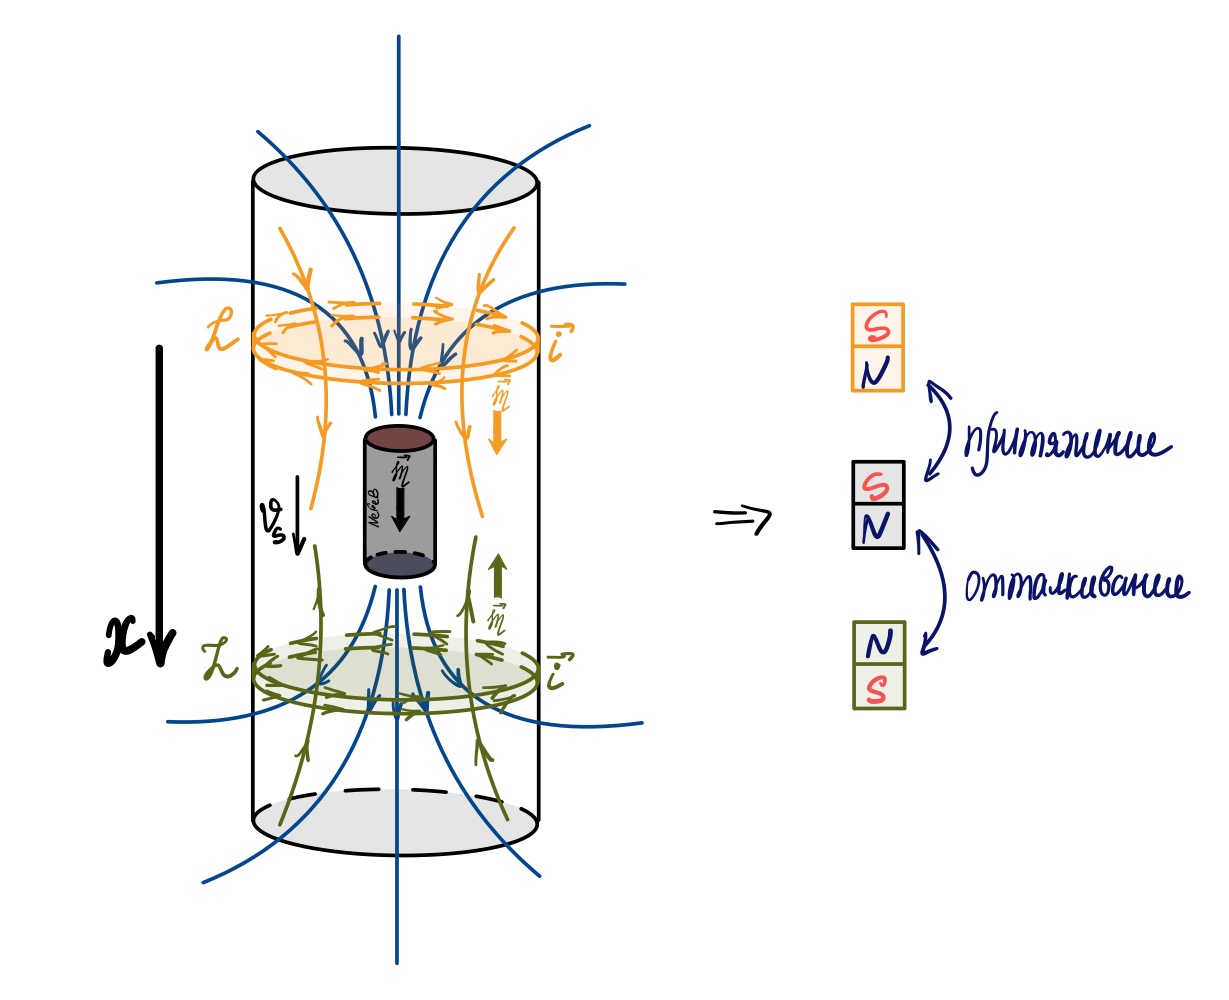
\includegraphics[scale=0.33]{1.JPG}
	\caption{К описанию явления}
\end{figure}

\newpage

%3
%=======================================================================================

\section{Теоретическая составляющая эксперимента}

Простейший магнитный диполь, в отличие от электрического (в силу отсутствия в природе магнитных зарядов), представляет собой тонкий замкнутый виток с током: $\overrightarrow{p_m} = I\overrightarrow{S},$ где $\overrightarrow{S} = S\overrightarrow{n}$ -- вектор площади контура, образующий с направлением тока правовинтовую систему (рис. 2а). По этой же
формуле определяется и магнитный момент соленоида, если под $I$ понимать полный ток, текущий по его боковой поверхности, а под $S$ -- площадь его поперечного сечения. Для проволочной цилиндрической спирали с малым шагом, состоящей из $N$ витков, магнитный момент определен как $p_m = NIS.$ Если же магнитный диполь иной природы, например, постоянный магнит, то для расчета полей его очень удобно представить в виде витка или трубки с азимутальным током $I = \dfrac{p_m}{S}$. Этот фиктивный ток называют током намагничивания. В качестве источника поля он ведёт себя так же, как и реальный ток (рис. 2б). 

Для нашего эксперимента рассмотрим постоянный магнит в форме цилиндра. Всякий постоянный магнит обладает некоторым магнитным моментом $p_m,$ направленным от южного $S$ к северному $N$ магнитному полюсу так, что линии магнитной индукции выходят из северного и входят в южный полюс. Момент складывается из магнитных моментов молекул намагниченного вещества: $\overrightarrow{p_m} = \sum\overrightarrow{p_i}$ и практически не изменяется под влиянием внешнего магнитного поля. Степень намагничивания характеризуется магнитным моментом единицы объёма $\overrightarrow{P_m}$, который называют вектором намагниченности. Для однородно намагниченного вещества $$\overrightarrow{P_m} = \dfrac{\overrightarrow{p_m}}{V} = \sum\dfrac{\overrightarrow{p_i}}{V}.$$

Молекулярные токи, связанные с магнитными моментами отдельных молекул, складываясь, образуют макроскопический ток намагничивания $I,$ циркулирующий по боковой поверхности цилиндрического магнита. Выясним связь величины тока намагничивания с величиной намагниченности вещества. Если по боковой поверхности цилиндра циркулирует ток намагничивания $I,$ то магнитный момент такого цилиндра $p_m = IS.$ Намагниченность $P_m = \dfrac{p_m}{V} = \dfrac{IS}{V} = \dfrac{IS}{Sl} = \dfrac{I}{l} = i$ -- линейная плотность поверхностного тока (здесь $V = Sl$ -- объём цилиндра).

Таким образом, если нам известна намагниченность $P_m$ цилиндрического магнита, то
мы можем рассчитать поле этого магнита, воспользовавшись формулами для поля соленоида, по поверхности которого течёт ток с поверхностной плотностью $i = P_m.$

\begin{figure}[h!]
	\centering
	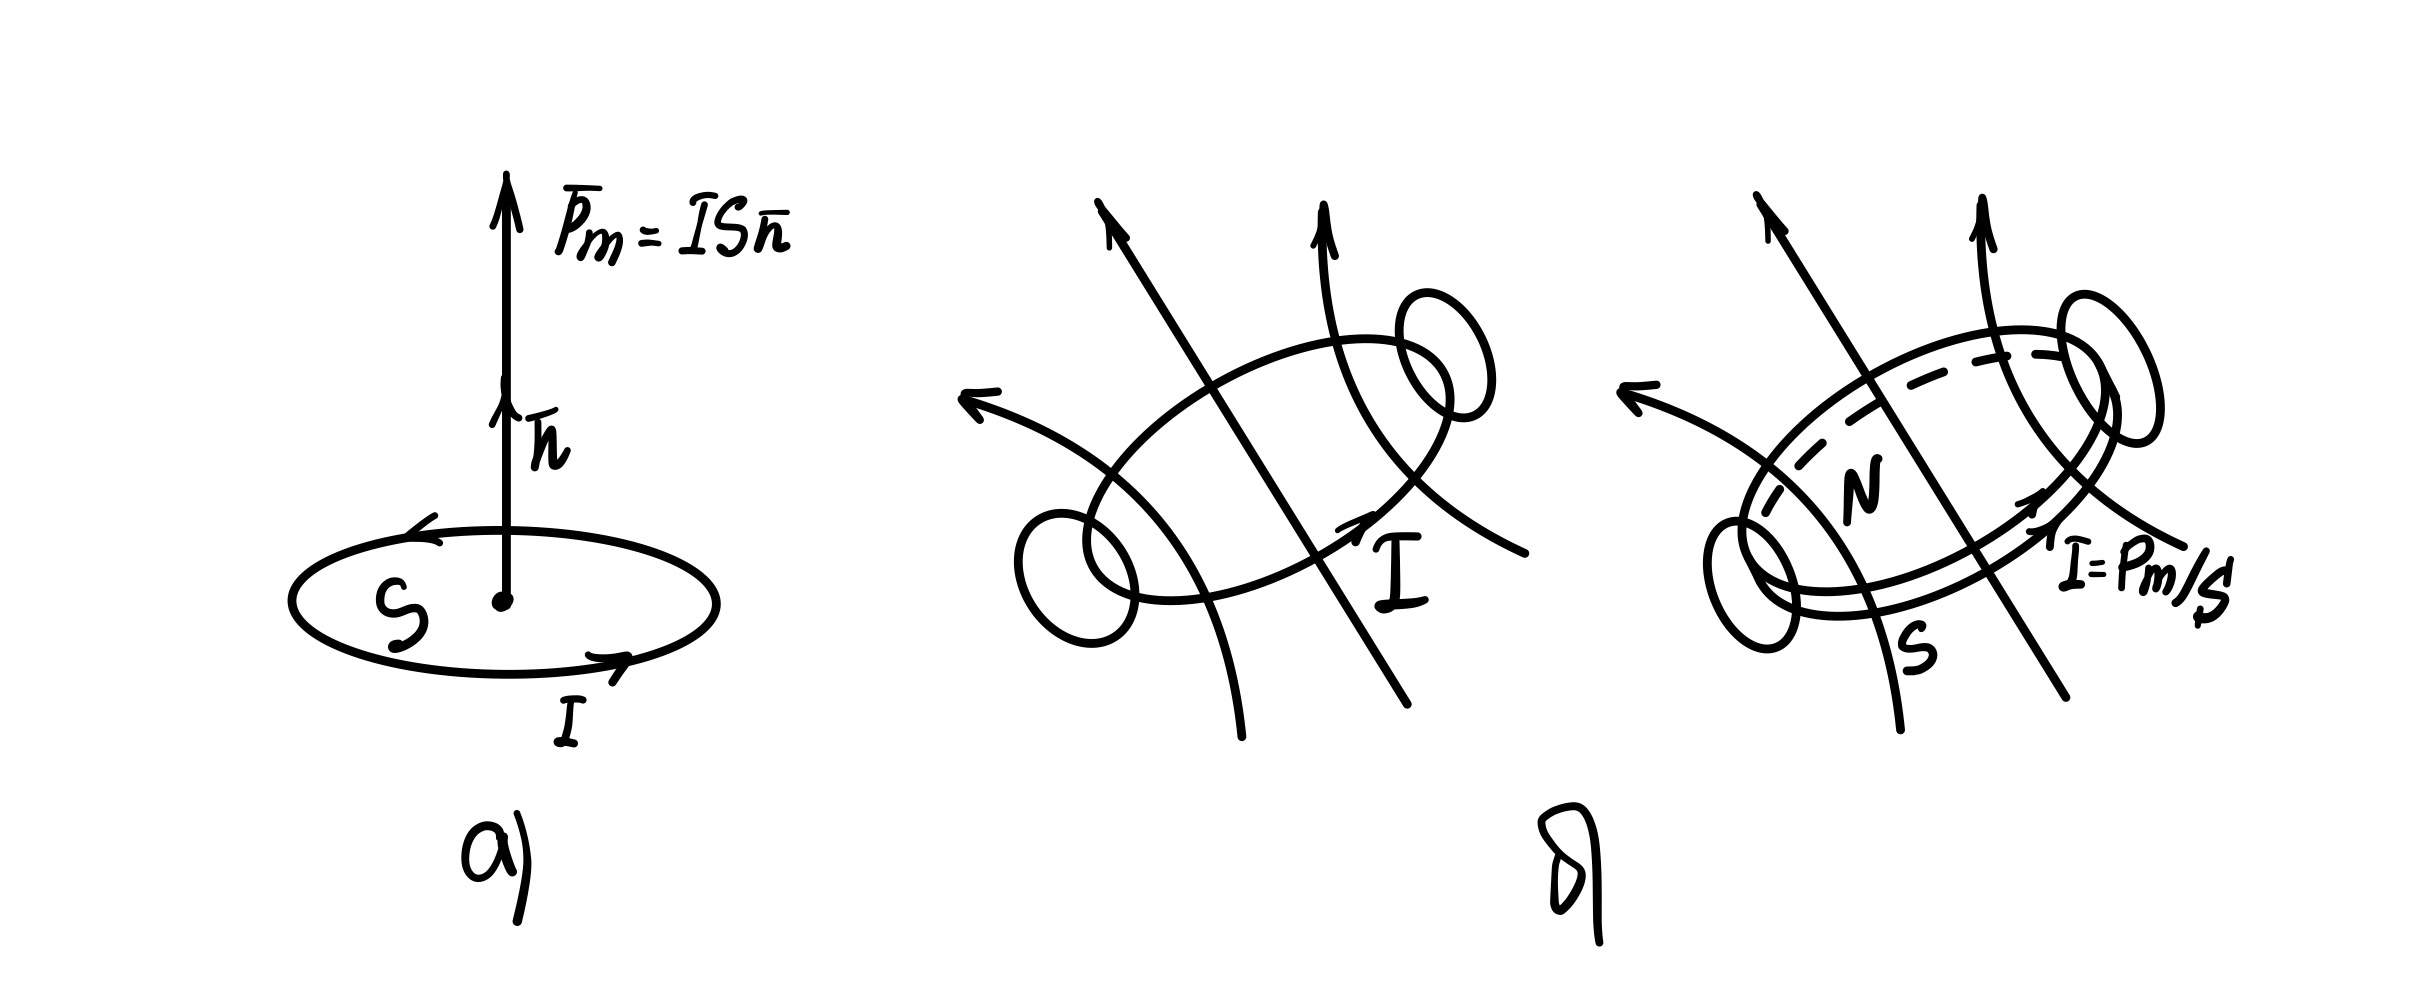
\includegraphics[scale=0.18]{2.JPG}
	\caption{Эквивалентность постоянного магнита витку с током}
\end{figure}

\newpage

Проведем сравнительный анализ для полей диполя и магнита на оси (для более детального рассмотрения в любой точке пространства вокруг магнита потребуются неоправданно сложные выкладки, поэтому ограничимся в сравнении только осью).

Поле соленоида на оси рассчитывается следующим образом (см. рис. 3):

\begin{figure}[h!]
	\centering
	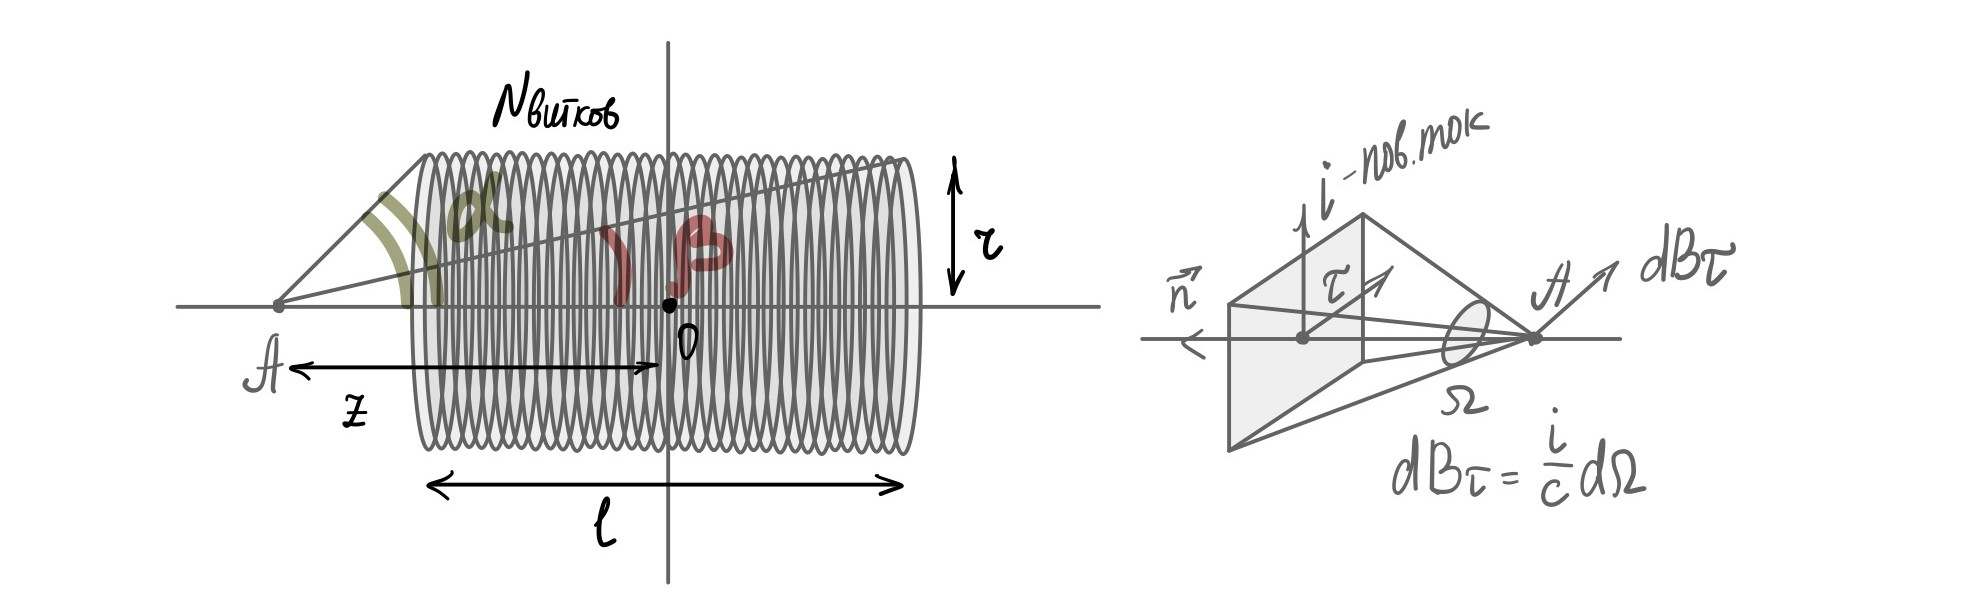
\includegraphics[scale=0.28]{4.JPG}
	\caption{К расчету поля соленоида на оси}
\end{figure}

$\Omega$ -- телесный угол, под которым видна внутренняя поверхность катушки. Тогда:
$$\Omega_1 = 2\pi(1 - cos\alpha)$$
$$\Omega_2 = 2\pi(1 - cos\beta)$$ 
$$\Omega = \Omega_1 - \Omega_2 = 2\pi - 2\pi cos\alpha - 2\pi + 2\pi cos\beta = 2\pi (cos\beta - cos\alpha)$$
$$dB_\tau = \dfrac{i}{c}d\Omega$$
$$i = \dfrac{IN}{l}$$
$$B_A = \dfrac{i}{c}\int d\Omega = \dfrac{i}{c}\Omega$$
$$B_A = \dfrac{IN}{lc} 2\pi (cos\beta - cos\alpha)$$

Теперь запишем поле эквивалетного магнита цилиндрической формы, полагая $i = P_m$, выразив косинусы углов через размерные параметры магнита и расстояние до точки наблюдения: 
$$B_A = \dfrac{P_m}{c} 2\pi \left(\dfrac{\dfrac{l}{2} + z}{\sqrt{r^2 + \left(\dfrac{l}{2} + z\right)^2}} - \dfrac{z - \dfrac{l}{2}}{\sqrt{r^2 + \left(z - \dfrac{l}{2}\right)^2}}\right)$$

С другой стороны, поле магнитного диполя с магнитным моментом $p_m$ на оси выражается следующим образом: $$B_A = \dfrac{2p_m}{z^3}$$

Предполагается, что зависимость магнитного поля на оси диполя от обратной величины кубического расстояния от середины магнита до точки оси будет линейной. Проверим, будут ли аппроксимироваться линейной функцией экспериментально снятые данные для магнита, который использовался в работе. Для этого построим график (см. рис. 4).

\begin{figure}[h!]
	\centering
	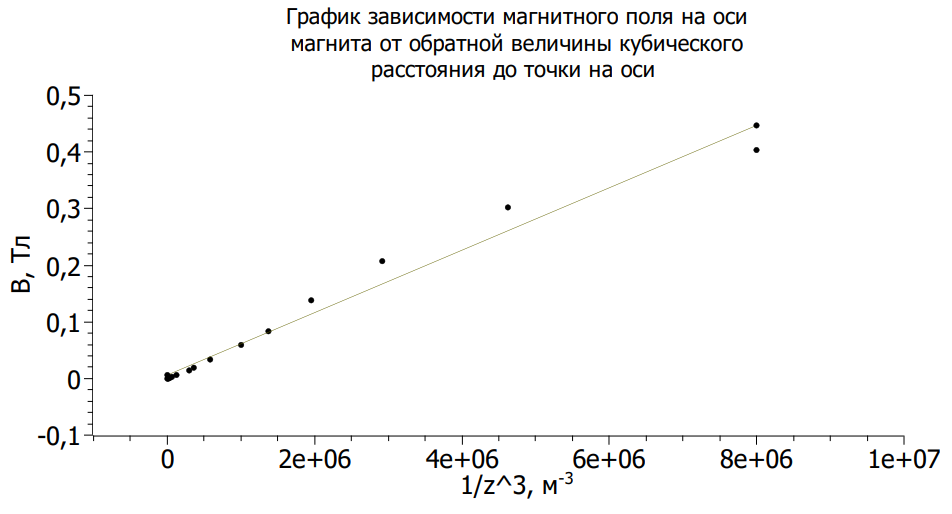
\includegraphics[scale=1,2]{6.png}
	\caption{К относительной эквивалентности полей диполя и магнита}
\end{figure}

Как видно из графика, незначительные отклонения от линейной зависимости позволяют утверждать, что с большой точностью поля можно считать эквивалентными.

Более того, можно сравнить функциональные коэффициенты в обеих формулах для индукции поля, построив их графики на одной плоскости и задав параметры экспериментального магнита. На рис. 5 можно видеть, что графики функций в нужном для эксперимента диапазоне значений хорошо ложатся друг на друга, поэтому можно смело упростить вычисления, заменив поле магнита полем диполя.

\begin{figure}[h!]
	\centering
	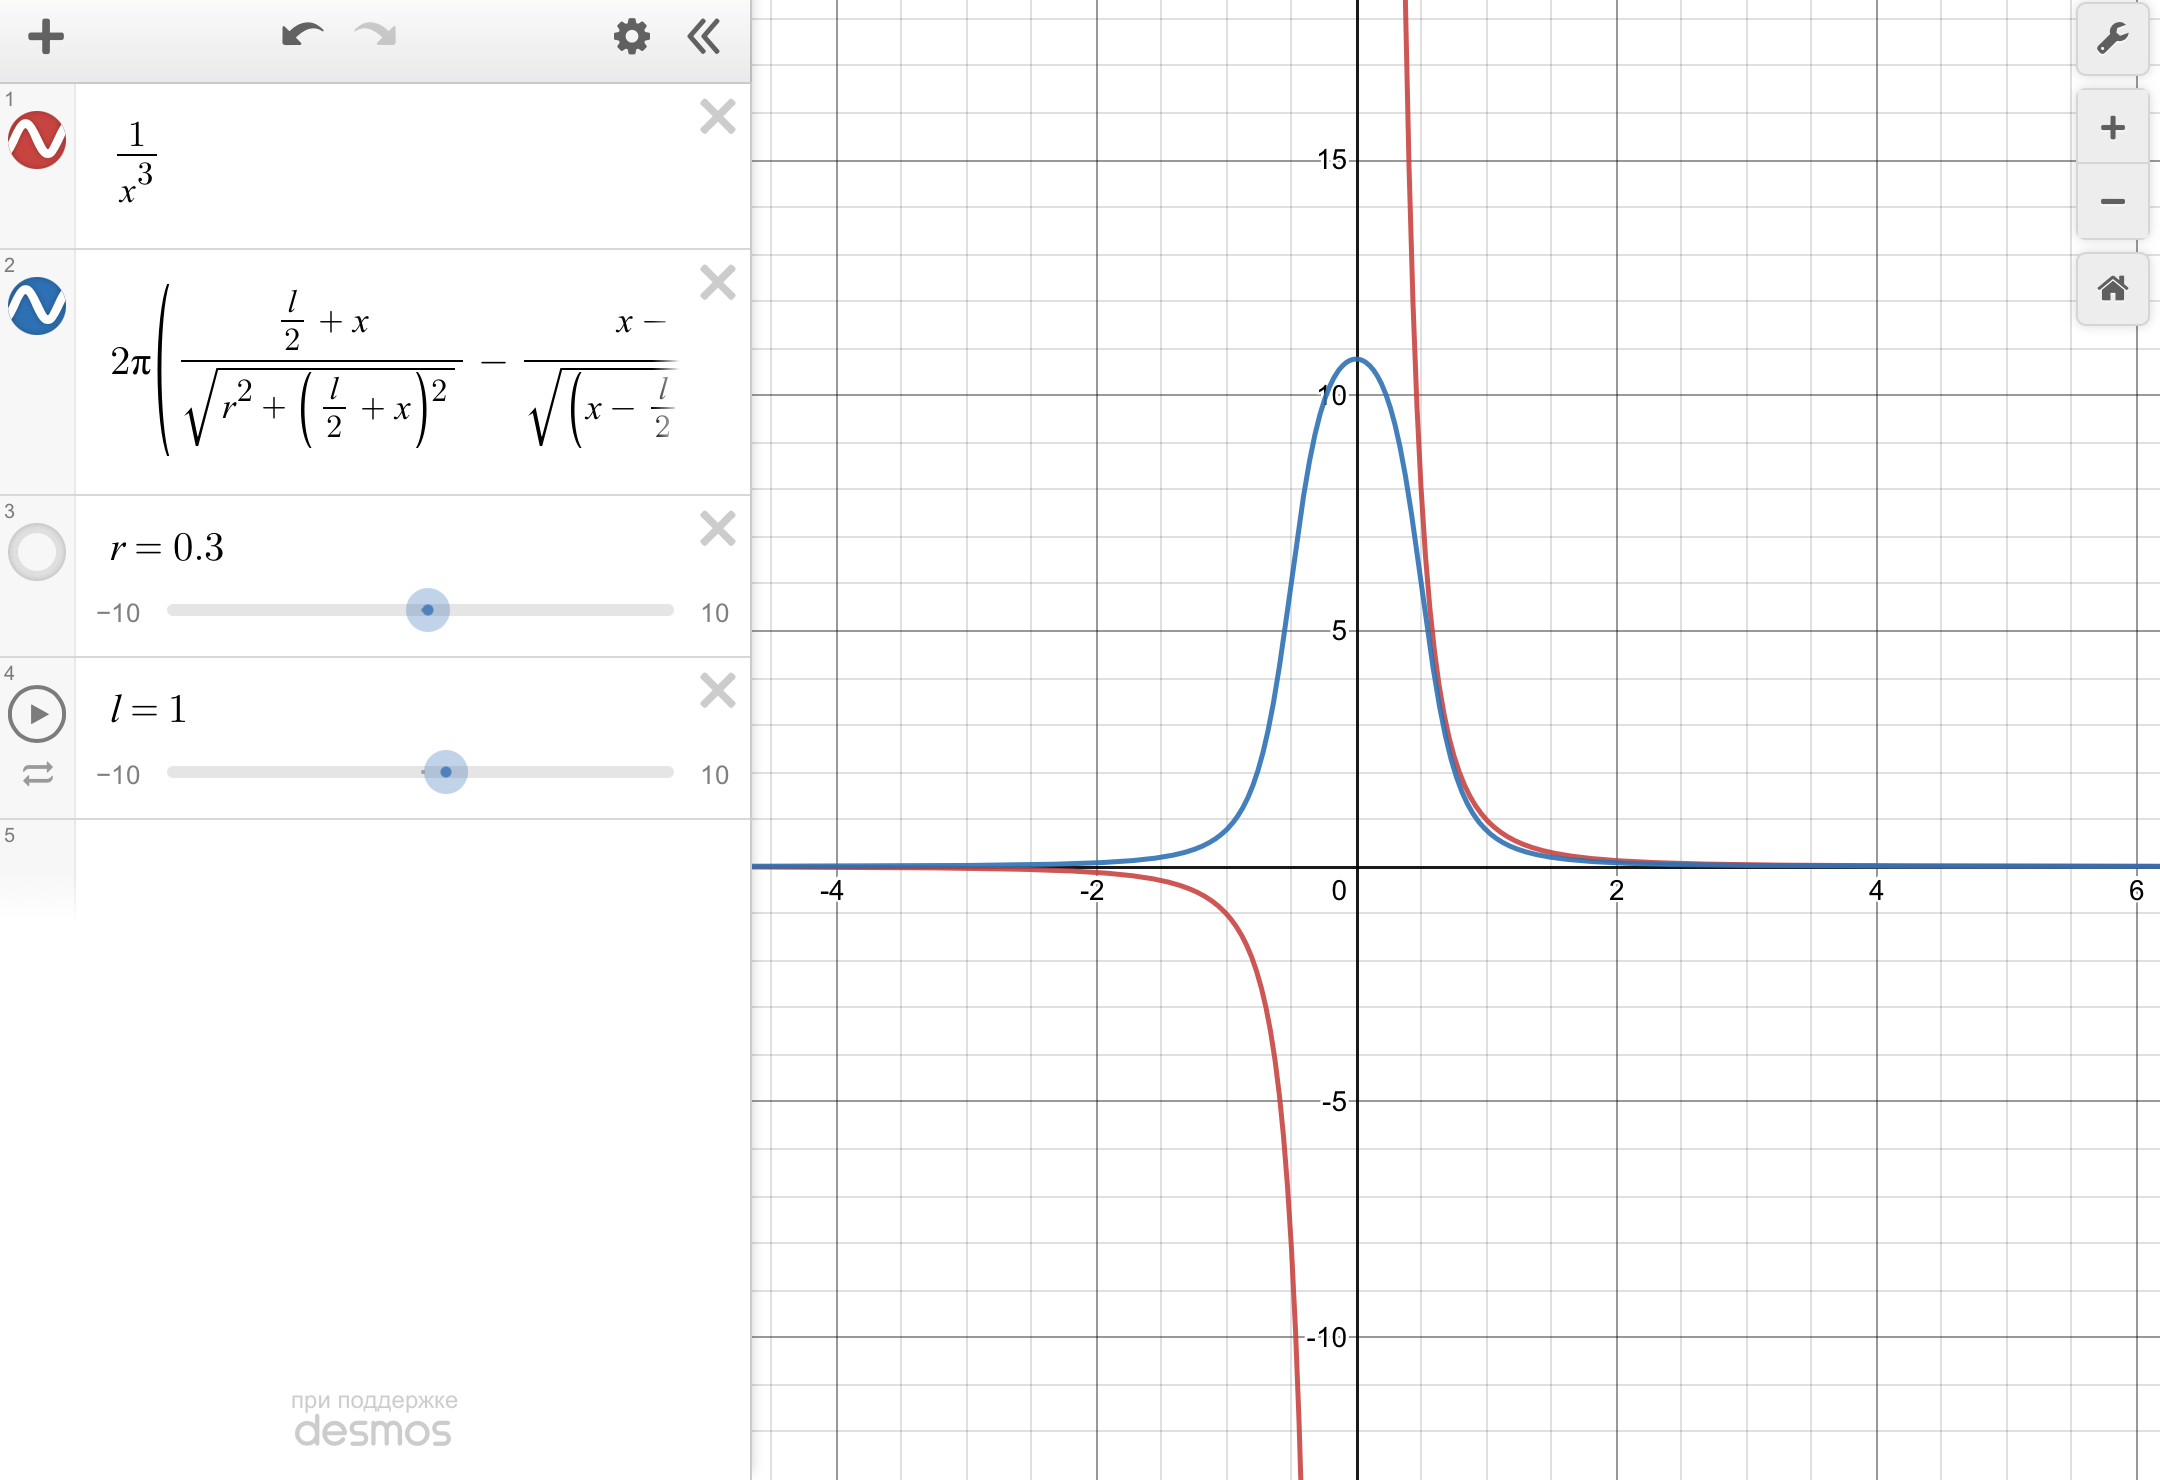
\includegraphics[scale=0.19]{5.PNG}
	\caption{К относительной эквивалентности полей диполя и магнита (2)}
\end{figure}

В дополнение приведем график (см. рис. 6) поля магнита на оси от расстояния (по форме он действительно похож на функции выше).

\begin{figure}[h!]
	\centering
	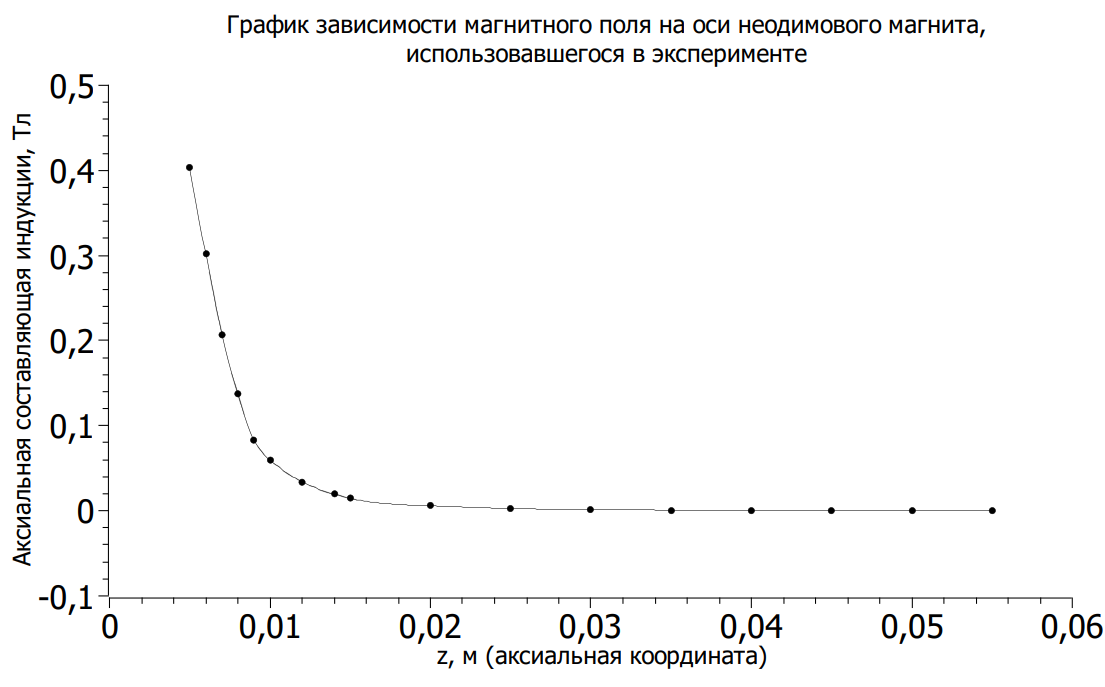
\includegraphics[scale=0.8]{испр.png}
	\caption{К относительной эквивалентности полей диполя и магнита (3)}
\end{figure}

После указания возможности аппроксимации поля на оси неодимового цилиндрического магнита полем диполя можно перейти к построению теории для последнего, проецируя ее с подразумевающимися, но негласными в этой работе поправками на реальное поле магнита. Дальнейшие выкладки будут приведены в СИ.

\begin{figure}[h!]
	\centering
	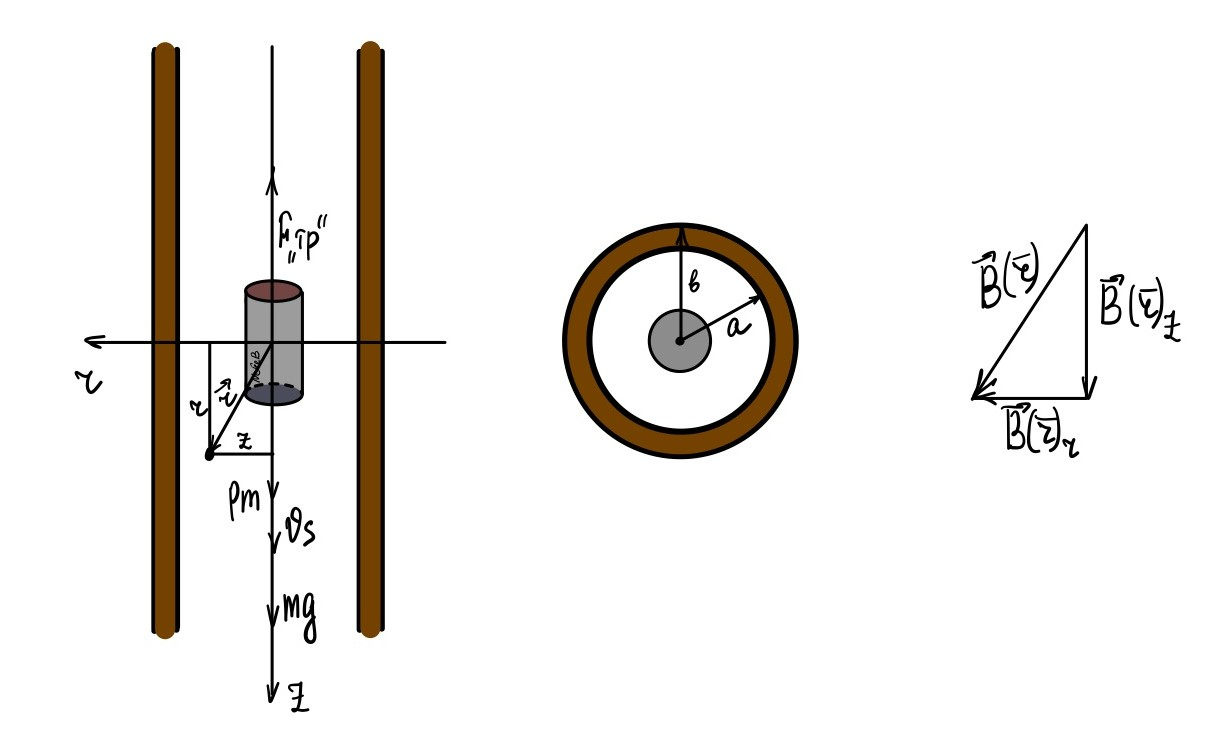
\includegraphics[scale=0.4]{3.JPG}
	\caption{К расчету установившейся скорости падения магнита}
\end{figure}

Введём координатные оси так, так показано на рис.7.
Примем обозначения: $\overrightarrow{r} = (r,z)$ -- радиус-вектор из центра диполя в точку наблюдения,\: $\overrightarrow{p_m}$ -- дипольный момент магнита.

Магнитное поле диполя: $$\overrightarrow{B} = \dfrac{\mu_0}{4\pi}\left(\dfrac{3(\overrightarrow{p_m} \overrightarrow{r})\overrightarrow{r}}{|\overrightarrow{r}|^5} - \dfrac{\overrightarrow{p_m}}{|\overrightarrow{r}|^3}\right)$$

Запишем z-компоненту магнитного поля диполя в зависимости от координат точки наблюдения (см. рис. 7), чтобы впоследствии вычислить магнитный поток, захваченный в поперечном сечении трубы: $$B_z(r,z) = \dfrac{\mu_0 p_m}{4\pi} \dfrac{2z^2 - r^2}{(r^2 + z^2)^\frac{5}{2}}$$

Для магнитного потока через площадь, охватываемую окружностью радиуса $r$ на расстоянии $z$ от диполя можно записать:
$$\Upphi(r,z) = \int\limits_{0}^{2\pi}\int\limits_{0}^{r}B_z(r^\prime,z) r^\prime d r^\prime d \phi = 2\pi \int\limits_{0}^{r}\dfrac{\mu_0 p_m}{4\pi}\dfrac{2z^2 - r^{\prime2}}{(r^{\prime 2} + z^2)^\frac{5}{2}} r^\prime dr^\prime.$$

После подсчета интеграла получим:
$$\Upphi(r,z) = \dfrac{\mu_0 p_m}{2}\dfrac{r^2}{(r^2 + z^2)^\frac{3}{2}}.$$

В силу движения диполя вдоль оси $z$ со скоростью $v$ сделаем следующую подстановку:
$$\Upphi(r,z) \rightarrow \Upphi(r, z - vt)$$

Запишем теперь 3-е уравнение Максвелла, говорящее от том, что изменение потока магнитной индукции, проходящего через незамкнутую поверхность $S$, взятое с обратным знаком, пропорционально циркуляции электрического поля на замкнутом контуре $L$, который является границей поверхности $S$:

$$\oint\limits_{L} \overrightarrow{E}d\overrightarrow{l} = -\dfrac{\partial}{\partial t}\int \overrightarrow{B} d\overrightarrow{S}$$

Тогда
$$2\pi rE(r, z) = -\dfrac{\partial}{\partial t}\Upphi(r, z - vt)$$

Выразим напряженность индуцированного электрического поля:
$$E(r,z) = -\dfrac{1}{2\pi r} \dfrac{\partial}{\partial t}\Upphi(r, z - vt) = -\dfrac{3\mu_0 p_m}{4\pi} \dfrac{rv(z - vt)}{(r^2 + (z - vt)^2)^\frac{5}{2}}$$

Теперь запишем закон Ома для текущих по поверхности трубы вихревых токов Фуко с плотностью $j$; проводимость меди -- $\lambda$:
$$\overrightarrow{j} = \lambda \overrightarrow{E}$$

Электрический ток вызывает омические потери внутри проводника. Иными словами, энергия рассеивается внутри проводника и переходит в форму тепла во всём объёме этого проводника. Объёмная плотность мощности омических потерь по определению: 
$$w = \overrightarrow{j} \overrightarrow{E} = \lambda E^2$$

С другой стороны, при движении магнита сверху вниз его потенциальная энергия в поле тяжести Земли уменьшается, но скорость движения при этом остаётся постоянной, то есть не растёт, как это происходит при свободном падении. Значит, потенциальная энергия магнита рассеивается внутри проводника. Условно примем силу, тормозящую магнит, за силу трения, рассеивающую потенциальную энергию магнита в тепло. Запишем теперь баланс мощности: скорость убывания потенциальной энергии магнита равна мощности омических потерь в проводнике (условно, магнит -- отдает, проводник -- забирает и греется):
$$\dfrac{dE_p}{dt} = P$$

$$E_p = -mgz$$ 
$$\dfrac{dE_p}{dt} = -mg\dot{z} = \int\limits_{V}wdV$$

Считая длину трубы бесконечной (в сравнении с магнитом), запишем:
$$mgv = \int\limits_{-\infty}^{\infty}\int\limits_{0}^{2\pi}\int\limits_{a}^{b}\lambda E^2 rdrd\phi dz$$

Интегрирование по азимутальному углу $\phi$ можно заменить просто домножением на $2\pi$ в силу аксиальной симметрии задачи. Порядок интегрирования в данном интеграле можно изменить и сначала проинтегрировать по $z$, а потом по $r$. При интегрировании по $z$ по бесконечным пределам можно отбросить слагаемое $-vt$. Тогда:
$$\int\limits_{-\infty}^{\infty}\dfrac{z^2 dz}{(r^2 + z^2)^5} = \dfrac{5\pi}{128r^7}$$

Для полной мощности омических потерь:
$$P = \dfrac{15}{1024} {\mu_0}^2{p_m}^2 \lambda \left(\dfrac{1}{a^3} - \dfrac{1}{b^3}\right)v^2 = kv^2$$

В предыдущем выражении обозначили за $k$ коэффициент условного трения:
$$k = \dfrac{15}{1024} {\mu_0}^2{p_m}^2 \lambda \left(\dfrac{1}{a^3} - \dfrac{1}{b^3}\right)$$

Тогда
$$mgv = kv^2$$
$$mg = kv$$

Окончательно имеем установившуюся скорость падения магнита в медной трубе:
$$v_s = \dfrac{mg}{k}$$

В дополнение, если записать уравнение движения магнита, то получится то же самое выражение, что и для полета парашютиста:
$$ma = mg - kv$$

$$\dot{v} + \dfrac{k}{m} v = g$$

$$v(t) = v_0 e^{-\alpha t} + v_s(1 - e^{-\alpha t})$$

$\alpha = k/m$ — коэффициент затухания. Характерное время выхода на установившийся режим падения — $\tau = \alpha^{-1}$. Начальная скорость — $v_0$, установившаяся скорость — $v_s$.

%4
%=======================================================================================

\section{Эксперимент}

Попробуем проверить теорию, которая была изложена выше. Возьмем 4 медных трубы разных диаметров с одинаковой толщиной стенок и проведем серию экспериментов по запуску магнита (на самом деле эксплуатировались 3 трубы, для 4-й токи Фуко фактически не индуцировались в силу большого радиуса трубы относительно магнита) (см. рис. 8). Данные сведены в таблицу (см. рис. 9).

\begin{figure}[ht]\center
\begin{tabular}{cc}
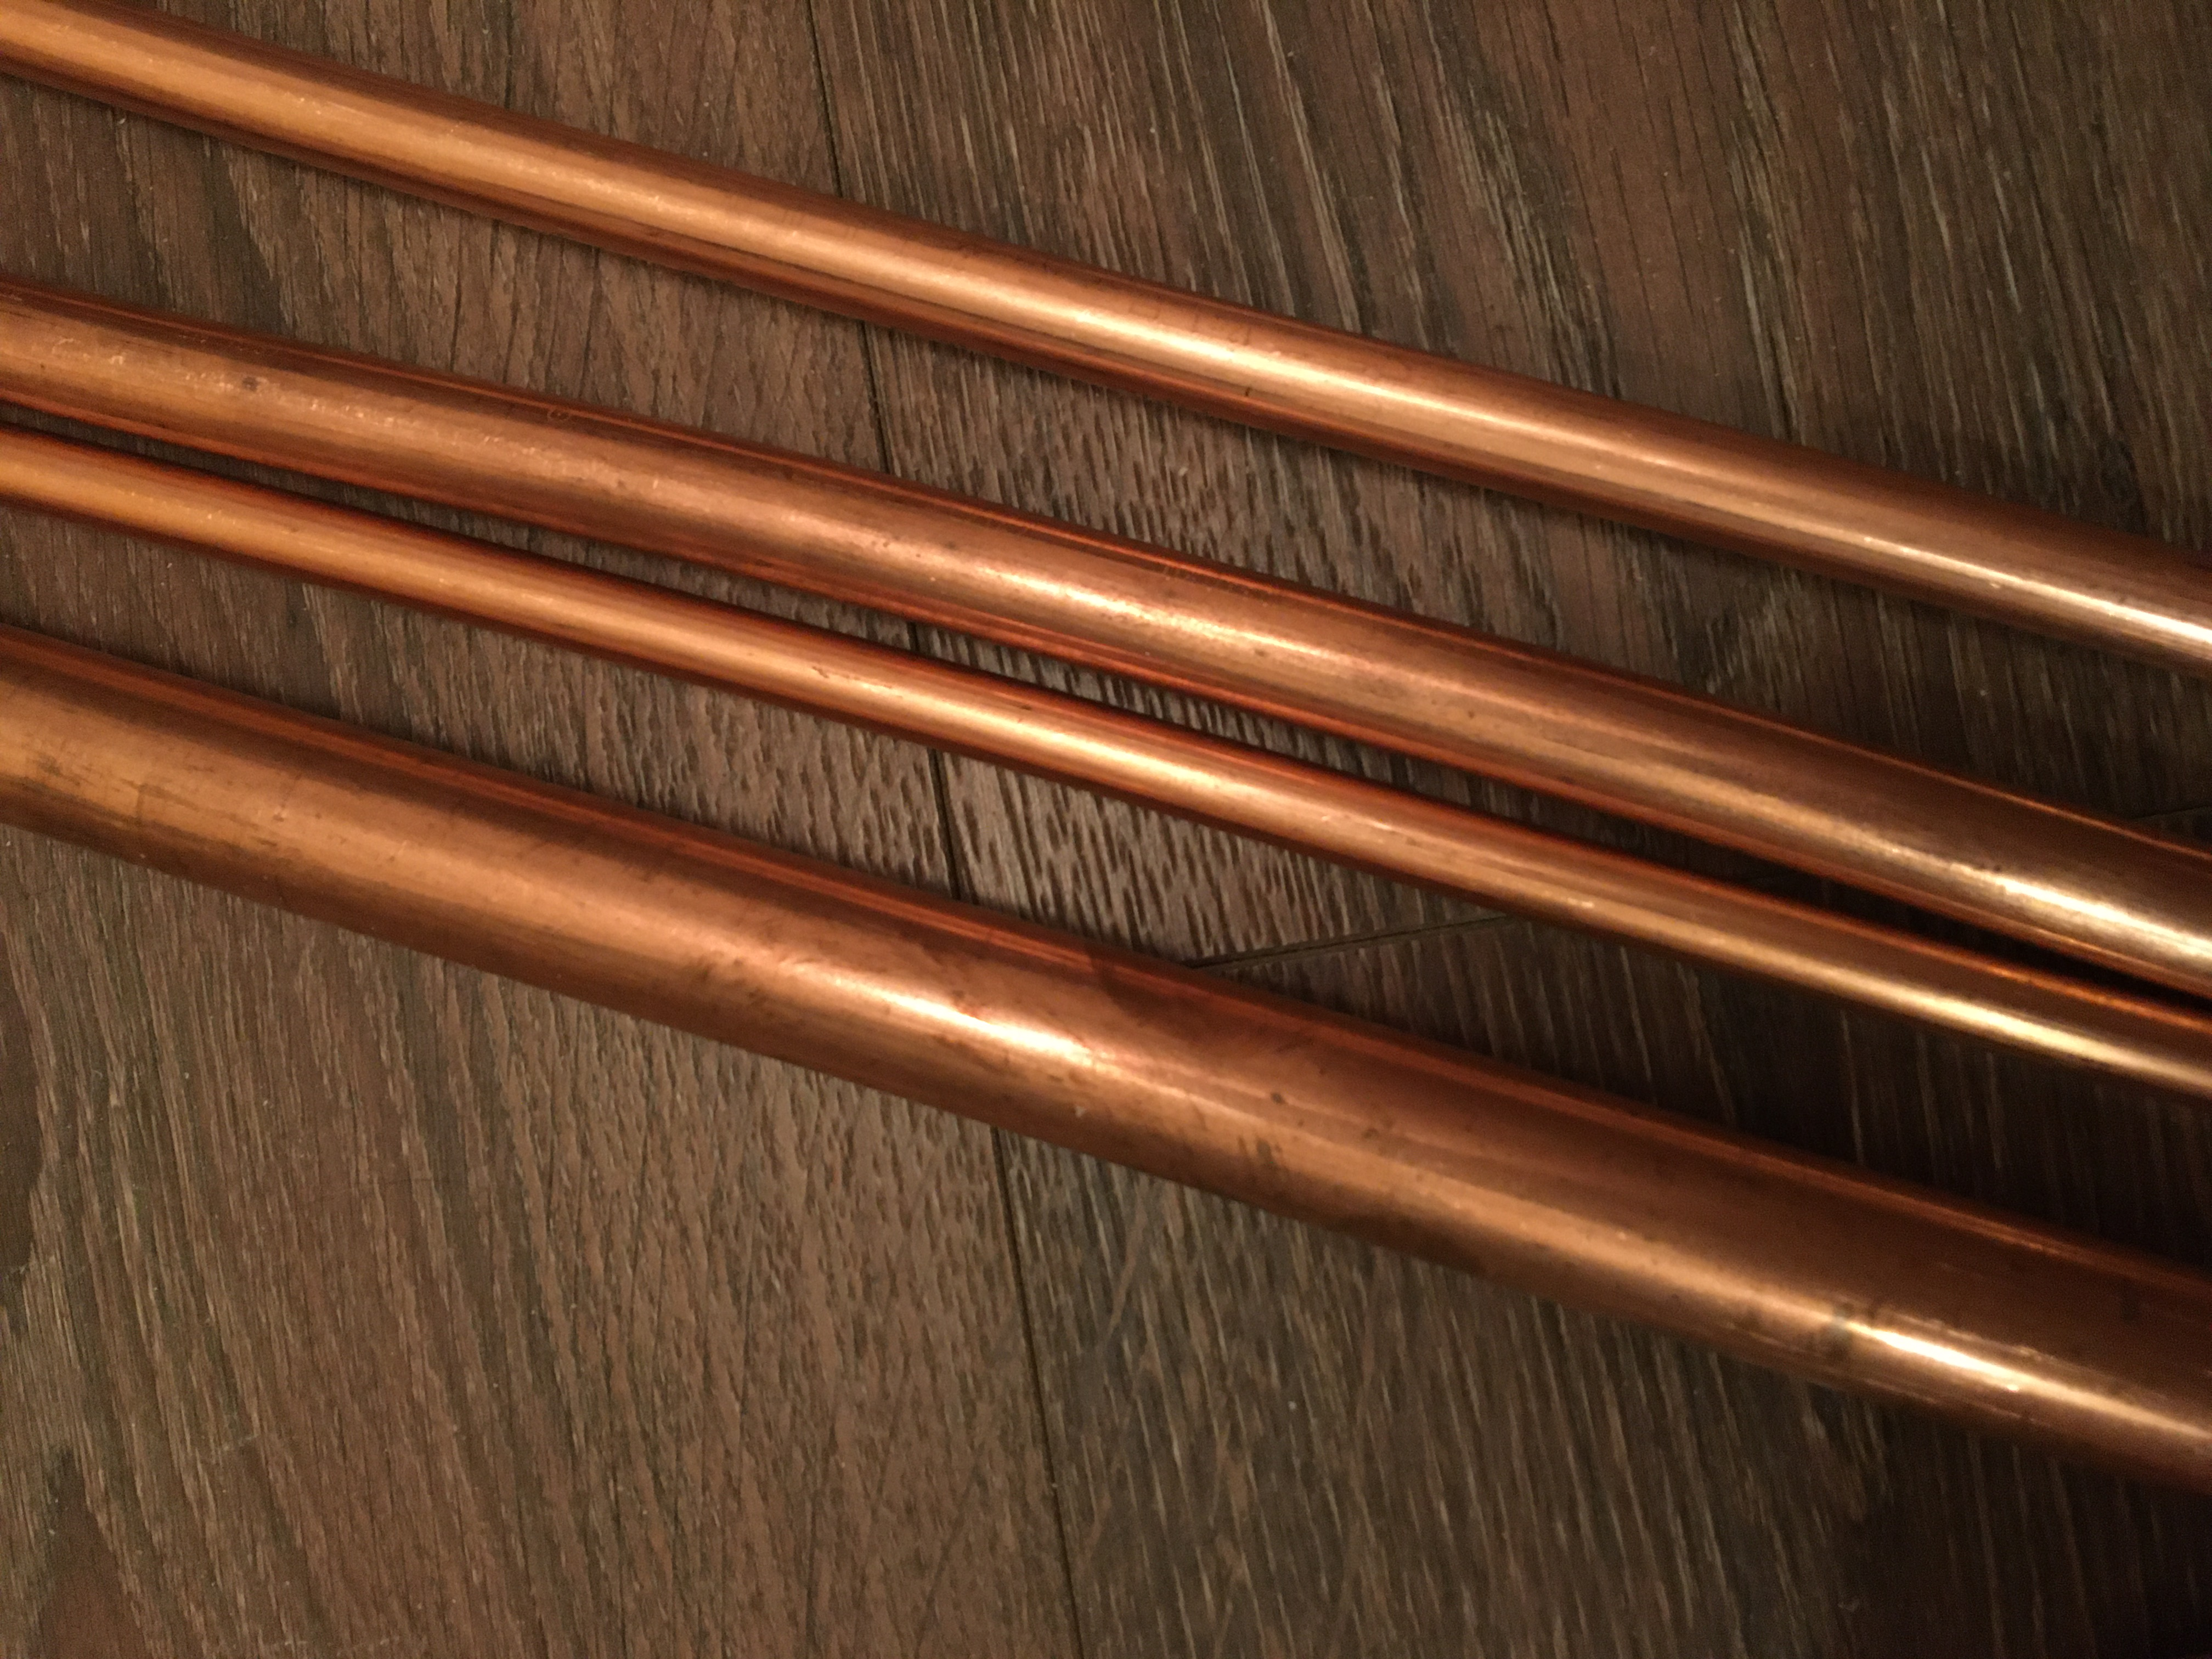
\includegraphics[width=80mm]{трубы.JPG}
&
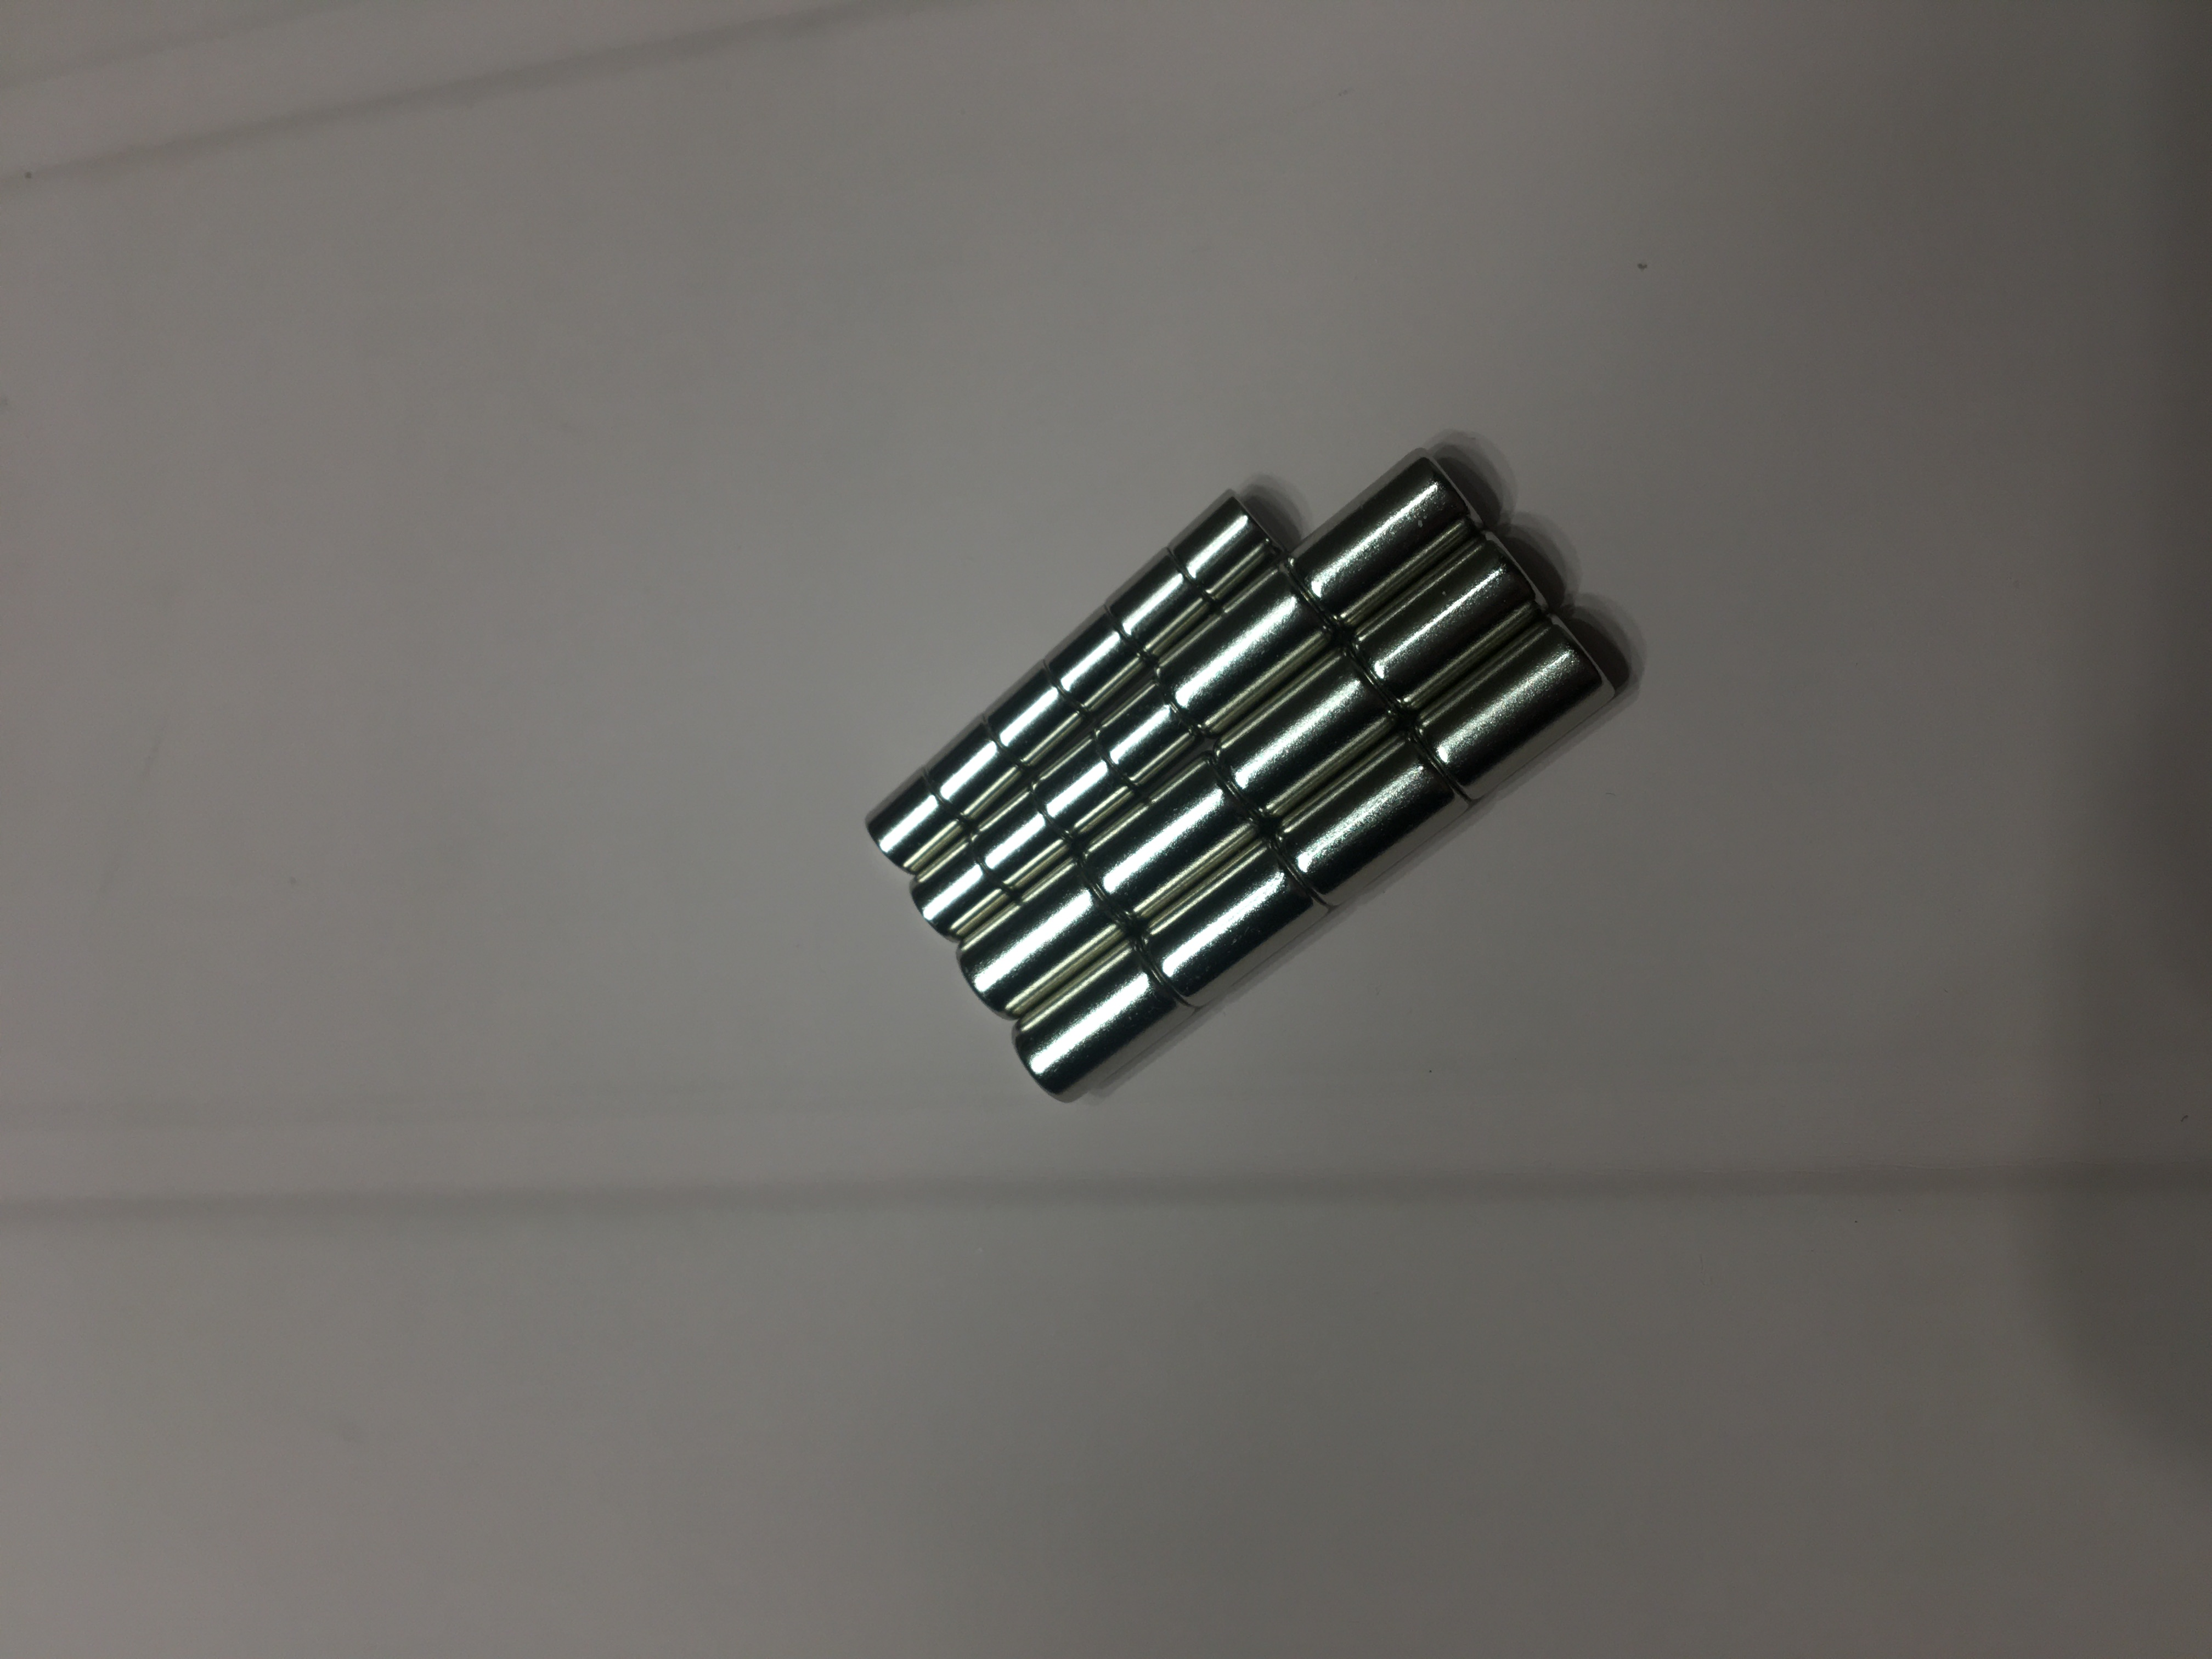
\includegraphics[width=80mm]{магниты.JPG}
\end{tabular}
\caption{Набор трубок и магнитов}
\end{figure}

Формулы и значения, использовавшиеся в расчетах:

$\mu_0 = 1,26\cdot10^{-6}$ H\cdot $А^2 = 4\pi \cdot 10^{-7}$ Гн/м

$\lambda = 59,52 \cdot 10^6$ 1/(Ом$\cdot$м)

$B = \mu \mu_0 H  = \mu_0(H + I)$

Здесь $I$ — вектор намагниченности вещества ($\equiv P_m$).

Известно, что для неодимовых магнитов остаточная намагниченность равна примерно $B_r = 1\,..\,1.3$ Т. Теперь, если исключить внешнее поле $H$ из предыдущего уравнения, получится
$B_r = \mu_0I$

Откуда находим магнитный момент, приходящийся на единицу объёма материала $I$ как
$I = \dfrac{B_r}{\mu_0}$

Чтобы найти магнитный момент магнита, нужно умножить $I$ на объём цилиндра $V$:

$p_m=IV=I\cdot\pi\left(\dfrac{d}{2}\right)^2 l = \dfrac{B_r}{\mu_0}\pi\left(\dfrac{d}{2}\right)^2 l$

Для $B_r = 1$ Тл результат расчета приведен в таблице.

При подсчете $k$ к результату прибавлялась небольшая поправка, связанная с коэффициентом трения магнита о воздух.

\begin{figure}[h!]
	\centering
	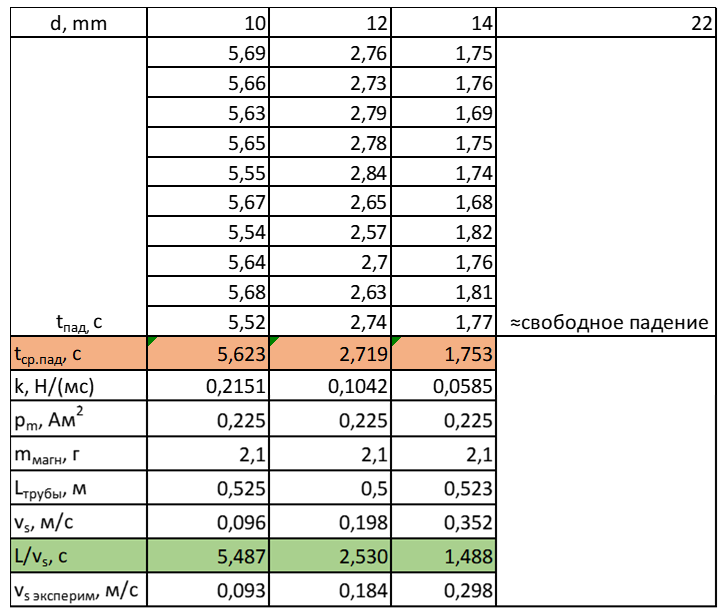
\includegraphics[scale=0.58]{фейл.png}
	\caption{Таблица результатов эксперимента}
\end{figure}

Нас интересуют значения двух выделенных строчек: рыжая - среднее экспериментальное время падения, зеленая - теоретический подсчет этого же времени, согласно теории предыдущего раздела.

Построим график зависимости теоретической и экспериментальной серии скоростей магнита в зависимости от диаметра труб (см. рис. 10).

\begin{figure}[h!]
	\centering
	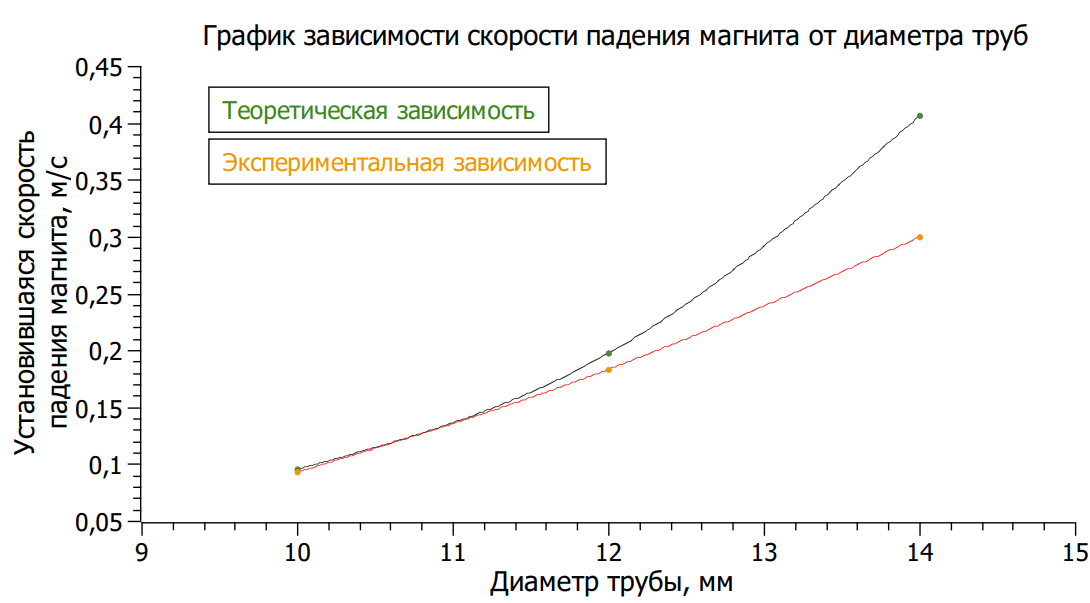
\includegraphics[scale=0.75]{граф.png}
	\caption{Скорость в зависимости от диаметра трубы}
\end{figure}

Проблемы, возникшие в ходе эксперимента, были связаны с запуском магнита в трубу так, чтобы он не тёрся о ее стенки, увеличивая тем самым время своего пролета и искажая данные. Из таблицы и графика видно, что труба с самым маленьким диаметром <<справилась>> лучше остальных, и результаты были все менее точными с ростом поперечного размера трубы. Дело в том, что по мере увеличения диаметральных размеров запускать магнит должным образом становилось все сложнее: иногда возникали перекручивания и механическое трение в силу слабеющих магнитных взаимодействий токов Фуко и летящего магнита. Более того, приходилось опускать магнит в трубу хотя бы на небольшое расстояние, чтобы ток успевал возникнуть и <<захватить>> магнит в правильном расположении. Расхождения в значениях также можно объяснить рядом замен на условно эквивалентные поля и скоростью реакции человека при замере времени.

\newpage

%5
%=======================================================================================

\section{Вывод}

В ходе данной работы было детально рассмотрено явление возникновения вихревых токов Фуко в медных трубах при пролете сквозь них неодимового магнита. Теория, разобранная в одном из разделов, успешно подтвердилась на практике, поэтому эксперимент можно считать удачно проведенным. 

P.S. Отдельная благодарность Бабинцеву Владимиру Александровичу за оказанную помощь.

\newpage

%8
%=======================================================================================

\section{Источники и ресурсы}

1. Д.В. Сивухин, "Общий курс физики". Учеб. пособие: Для вузов. В 5 т. Т.III. Электричество.

2. Научно-популярный физико-математический журнал <<Квант>>, №1, январь 2021, стр. 50-52.

3. http://imlab.narod.ru/M_Fields/A_Magnet/A_Magnet.htm

4. https://habr.com/ru/post/490310/

5. https://mipt.ru/education/chair/physics/kmf/mPh_5/f_5tlro8/f_5tlru2.pdf

\end{document}